\documentclass[aspectratio=169]{beamer}

% Shared Beamer settings for Applied Machine Learning lectures (UPES).
% Keep this file free of \documentclass to allow reuse via \input.

% Allow lecture sources to use shared theme/assets without copying them into each lecture folder.
% NOTE: These paths are relative to `Unit-xx/Lecture-yy/latex/` (and `Lab/Experiment-xx/latex/`).
\makeatletter
\def\input@path{{../../../_shared/}{../../../_shared/UPES-Beamer-Theme/}}
\makeatother

\usetheme{UPES}
\setbeamertemplate{navigation symbols}{}

\usepackage{amsmath}
\usepackage{amssymb}
\usepackage{booktabs}
\usepackage{graphicx}
\usepackage{hyperref}
\usepackage{xcolor}
\usepackage{listings}

% Code listings (Python-oriented for this subject).
\lstset{
  language=Python,
  basicstyle=\ttfamily\small,
  keywordstyle=\color{blue},
  commentstyle=\color{gray},
  stringstyle=\color{teal},
  showstringspaces=false,
  columns=fullflexible,
  breaklines=true
}

\usepackage{tikz}
\usetikzlibrary{arrows.meta,positioning,shapes.geometric,calc,fit,backgrounds}

% Per-slide source line (references shown on the slide itself).
\newcommand{\slidesources}[1]{%
  \vfill
  {\tiny\color{gray}\raggedright\sloppy\parbox{\linewidth}{Sources: #1}\par}%
}

% Unit-wise source strings for this subject (used by slides/notes).
% Path is relative to the lecture `latex/` folder (the compilation CWD).
% Source strings for Applied Machine Learning (CSAI2017P) — used by slides + notes.
% Prescribed texts and reference books are taken from the course syllabus.
% Support texts are the author-hosted open-access editions:
%   statlearning.com            (ISL with Python)
%   probml.github.io/pml-book   (Murphy, Probabilistic Machine Learning)
%   d2l.ai                      (Dive into Deep Learning)
%   mml-book.github.io          (Mathematics for Machine Learning)

\newcommand{\AMLRepoURL}{https://github.com/tali7c/Applied-Machine-Learning}

% --- prescribed -------------------------------------------------------------
\newcommand{\AMLPrescribed}{%
M\"uller and Guido, \textit{Introduction to Machine Learning with Python}, O'Reilly, 2016.;%
Bishop, \textit{Pattern Recognition and Machine Learning}, Springer, 2006.;%
Murphy, \textit{Machine Learning: A Probabilistic Perspective}, MIT Press, 2012.;%
Han, Kamber and Pei, \textit{Data Mining: Concepts and Techniques} (3e), Morgan Kaufmann, 2012.%
}

% --- unit-wise ---------------------------------------------------------------
\newcommand{\AMLUnitISources}{%
M\"uller and Guido, \textit{Introduction to Machine Learning with Python}, Ch. 1.;%
Bishop, \textit{Pattern Recognition and Machine Learning}, Ch. 1.;%
Murphy, \textit{Probabilistic Machine Learning: An Introduction}, MIT Press, 2022, Ch. 1.;%
Mitchell, \textit{Machine Learning}, McGraw Hill, 1997, Ch. 1.;%
Scikit-learn documentation, accessed 2026-08-04.%
}

\newcommand{\AMLUnitIISources}{%
Bishop, \textit{Pattern Recognition and Machine Learning}, \S1.5, \S4.3, \S7.1.;%
Zhang, Lipton, Li and Smola, \textit{Dive into Deep Learning}, \S3.4.;%
Shalev-Shwartz and Ben-David, \textit{Understanding Machine Learning}, Ch. 15.;%
Murphy, \textit{Probabilistic Machine Learning: An Introduction}, Ch. 5.%
}

\newcommand{\AMLUnitIIISources}{%
Zhang, Lipton, Li and Smola, \textit{Dive into Deep Learning}, Ch. 12 (Optimization Algorithms).;%
Deisenroth, Faisal and Ong, \textit{Mathematics for Machine Learning}, Ch. 7.;%
Kingma and Ba, ``Adam: A Method for Stochastic Optimization,'' ICLR 2015.;%
Ruder, ``An overview of gradient descent optimization algorithms,'' arXiv:1609.04747, 2016.%
}

\newcommand{\AMLUnitIVSources}{%
Han, Kamber and Pei, \textit{Data Mining: Concepts and Techniques} (3e), Ch. 3.;%
M\"uller and Guido, \textit{Introduction to Machine Learning with Python}, Ch. 3--4.;%
James, Witten, Hastie, Tibshirani and Taylor, \textit{An Introduction to Statistical Learning with Python}, Ch. 5--6, 12.;%
Scikit-learn documentation (preprocessing, model selection), accessed 2026-08-04.%
}

\newcommand{\AMLUnitVSources}{%
James et al., \textit{An Introduction to Statistical Learning with Python}, Ch. 3--6.;%
Bishop, \textit{Pattern Recognition and Machine Learning}, Ch. 3.;%
Deisenroth, Faisal and Ong, \textit{Mathematics for Machine Learning}, Ch. 9.;%
M\"uller and Guido, \textit{Introduction to Machine Learning with Python}, \S2.3.%
}

\newcommand{\AMLUnitVISources}{%
Han, Kamber and Pei, \textit{Data Mining: Concepts and Techniques} (3e), Ch. 8--9.;%
James et al., \textit{An Introduction to Statistical Learning with Python}, Ch. 8--9.;%
Bishop, \textit{Pattern Recognition and Machine Learning}, Ch. 4--5, 7, 14.;%
Zhang et al., \textit{Dive into Deep Learning}, Ch. 5.%
}

\newcommand{\AMLUnitVIISources}{%
Han, Kamber and Pei, \textit{Data Mining: Concepts and Techniques} (3e), Ch. 10.;%
James et al., \textit{An Introduction to Statistical Learning with Python}, Ch. 12.;%
M\"uller and Guido, \textit{Introduction to Machine Learning with Python}, \S3.5.;%
Ester, Kriegel, Sander and Xu, ``A density-based algorithm for discovering clusters (DBSCAN),'' KDD 1996.%
}

\newcommand{\AMLLabSources}{%
M\"uller and Guido, \textit{Introduction to Machine Learning with Python}, companion notebooks.;%
McKinney, \textit{Python for Data Analysis} (3e), O'Reilly, 2022.;%
Scikit-learn user guide, accessed 2026-08-04.;%
Matplotlib and Seaborn documentation, accessed 2026-08-04.%
}



\graphicspath{{../figures/}{../images/}{../../../_shared/}{../../../_shared/UPES-Beamer-Theme/}}

\title[Applied Machine Learning]{Applied Machine Learning}
\subtitle{Unit 03 -- Lecture 04: Adaptive Optimisers}
\author{Tofik Ali}
\institute{School of Computer Science, UPES Dehradun}
\date{Autumn 2026}

% ---- a compact "output" block so code and its result sit together ----------
\lstdefinestyle{outblk}{
  basicstyle=\ttfamily\scriptsize\color{black!75},
  backgroundcolor=\color{black!5}, frame=leftline, framerule=2pt,
  rulecolor=\color{black!30}, breaklines=true, columns=fullflexible,
  keepspaces=true,   % several outputs below are aligned tables
  language={},       % printed output is not Python: do not syntax-highlight it
  xleftmargin=4pt, aboveskip=1pt, belowskip=1pt, literate={-}{{-}}1}
\lstnewenvironment{outblk}{\lstset{style=outblk}}{}

\begin{document}

\UPESCoverFrame
\setcounter{framenumber}{0}

\begin{frame}
  \titlepage
  \vspace{0.3em}
  \begin{center}
    \footnotesize Adagrad, RMSprop, Adadelta, Adam --- and numerical practice\\[0.25em]
    \footnotesize Topic focus: \textbf{what if every parameter needs its own
      learning rate?}\\[0.25em]
    \footnotesize Repository: \texttt{\AMLRepoURL}
  \end{center}
  \slidesources{\AMLUnitIIISources}
\end{frame}

\begin{frame}{Quick Links}
  \centering
  \hyperlink{sec:why}{\beamerbutton{One rate is not enough}}\hspace{0.4em}
  \hyperlink{sec:adagrad}{\beamerbutton{Adagrad}}\hspace{0.4em}
  \hyperlink{sec:rmsprop}{\beamerbutton{RMSprop}}\hspace{0.4em}
  \hyperlink{sec:adadelta}{\beamerbutton{Adadelta}}\hspace{0.4em}
  \hyperlink{sec:adam}{\beamerbutton{Adam}}\hspace{0.4em}
  \hyperlink{sec:practice}{\beamerbutton{Practice}}\hspace{0.4em}
  \hyperlink{sec:summary}{\beamerbutton{Summary}}
\end{frame}

\begin{frame}{Agenda}
  \tableofcontents
\end{frame}

\begin{frame}[shrink=6]{How this lecture works}
  \begin{columns}[T]
    \begin{column}{0.48\textwidth}
      \begin{block}{Every idea appears twice}
        \begin{enumerate}
          \item \textbf{By hand} --- four optimisers worked on the same little
            bowl $f(w)=(w-3)^2$, so you can compare them line by line.
          \item \textbf{In code} --- the same arithmetic, so you see the library
            does exactly that and nothing magic.
        \end{enumerate}
      \end{block}
    \end{column}
    \begin{column}{0.48\textwidth}
      \begin{alertblock}{Commit before you look}
        Five slides ask you to predict an answer before it is revealed. Write
        your guess down. Being wrong on paper is how the idea sticks.
      \end{alertblock}
    \end{column}
  \end{columns}
  \vspace{0.4em}
  \begin{center}
    \small The centrepiece is \textbf{three steps of Adam by hand}. Everything
    before it exists to make those three steps obvious.
  \end{center}
\end{frame}

\begin{frame}[fragile,shrink=10]{Two Datasets, One Seed}
  \begin{block}{The convention, and a distinction worth keeping}
    \small
    \begin{itemize}
      \item \textbf{One seed: 1.} Every mini-batch shuffle and every
        gradient-noise draw today is \texttt{np.random.default\_rng(1)},
        shown in the listing, never hidden in a helper.
      \item The sparse-feature problem is built with a \emph{different} fixed
        number --- and that is not sloppiness.
    \end{itemize}
  \end{block}
  \begin{alertblock}{A shuffle seed and a dataset seed are not the same thing}
    \small Change the \textbf{shuffle} seed and you get another run of the same
    experiment. Change the \textbf{dataset} seed and you get a different
    experiment. Give them the same name and someone eventually ``tidies up''
    by unifying them --- and silently deletes the demonstration.
  \end{alertblock}
  {\footnotesize Every number in these slides reproduces exactly. Differ, and
  it is your code or your library version --- not luck.}
\end{frame}

\begin{frame}[shrink=5]{Where we are}
  \begin{columns}[T]
    \begin{column}{0.47\textwidth}
      \begin{block}{The last lecture gave us}
        $w \leftarrow w - \eta\,\nabla J$, the ceiling $\eta < 2/L$, mini-batches,
        and momentum $v \leftarrow \beta v + g$.
      \end{block}
      \begin{block}{It also gave us the villain}
        On \texttt{load\_diabetes}: largest curvature $8.05$, smallest $0.017$,
        so $\kappa = 470$. Momentum cut $1605$ iterations to $128$.
      \end{block}
    \end{column}
    \begin{column}{0.49\textwidth}
      \begin{exampleblock}{Today's question}
        Momentum gives every coordinate the \textbf{same} $\eta$ and the
        \textbf{same} $\beta$.\\[0.3em]
        What if each coordinate needs its own step size --- and the algorithm
        has to work it out for itself?
      \end{exampleblock}
      \begin{alertblock}{Four answers, in historical order}
        Adagrad (2011) $\rightarrow$ RMSprop (2012) $\rightarrow$
        Adadelta (2012) $\rightarrow$ Adam (2015).
      \end{alertblock}
    \end{column}
  \end{columns}
\end{frame}

% =====================================================================
\section[One rate]{One learning rate is not enough}
\label{sec:why}

\begin{frame}[shrink=6]{What momentum does not fix}
  \begin{itemize}
    \item<1-> Momentum changes the \textbf{direction} it steps in --- an
      average of recent gradients instead of the current one.
    \item<2-> It does not change the \textbf{scale}. One $\eta$ still multiplies
      every coordinate of that average.
    \item<3-> So the ceiling is still set by the steepest direction, and the
      shallow directions still crawl.
  \end{itemize}
  \vspace{0.7em}
  \onslide<4->{
  \begin{exampleblock}{The idea of this whole lecture, in one line}
    \centering \Large
    $w_i \leftarrow w_i - \dfrac{\eta}{\sqrt{s_i}}\,g_i$
  \end{exampleblock}}
  \vspace{0.3em}
  \onslide<5->{
  \begin{center}\small
    Divide each coordinate's step by something that measures \textbf{how big
    that coordinate's gradients have been}. Every optimiser today differs only
    in what $s_i$ is.
  \end{center}}
\end{frame}

\begin{frame}[shrink=6]{By hand: two coordinates want two different step sizes}
  Take the ravine from last time, $f(w) = 0.01 w_1^2 + 2 w_2^2$. The Hessian is
  diagonal:
  \[
    H = \begin{pmatrix} 0.02 & 0 \\ 0 & 4 \end{pmatrix},
    \qquad \kappa = \frac{4}{0.02} = 200 .
  \]
  \begin{center}\small
  \begin{tabular}{@{}lrrl@{}}
    \toprule
    & curvature $\lambda_i$ & \emph{ideal} step $1/\lambda_i$ & \\
    \midrule
    $w_1$ (shallow) & $0.02$ & $50.0$ & wants a huge step\\
    $w_2$ (steep)   & $4.00$ & $0.25$ & wants a tiny one\\
    \bottomrule
  \end{tabular}
  \end{center}
  \vspace{0.3em}
  \begin{alertblock}{One number cannot be both}
    \small A single $\eta$ must satisfy $\eta < 2/4 = 0.5$ or $w_2$ diverges.
    That is $200\times$ smaller than what $w_1$ wants. \textbf{The condition
    number is exactly the size of the mismatch.}
  \end{alertblock}
\end{frame}

\begin{frame}[fragile,shrink=6]{A problem where one $\eta$ genuinely cannot work}
$40$ synthetic features, all with true weight exactly $1$. Twenty are dense;
twenty fire in progressively fewer rows.
\begin{lstlisting}
rng  = np.random.default_rng(0)             # fixes THE DATA, not a run
dens = np.geomspace(0.25, 0.005, 20)        # how often each rare one fires
for j in range(20):
    hit = rng.random(N) < dens[j]
    Xs[hit, 20 + j] = rng.standard_normal(hit.sum())
\end{lstlisting}
\begin{outblk}
rows                       4000
dense features, non-zero in 4000 to 4000 rows
rarest feature, non-zero in 18 rows
condition number  kappa    3.781e+02
every true weight is exactly 1.0
\end{outblk}
\begin{center}\small
  A rare feature contributes to a mini-batch gradient in maybe \emph{one} row
  out of $4000$. Its gradient is almost always zero.
\end{center}
\end{frame}

\begin{frame}[fragile]{Predict first \#1}
Plain SGD, $\eta = 0.01$, ten epochs, mini-batch $B=32$. Every true weight is
$1.0$, and the training MSE does come down to $0.085$.

\begin{center}
  \textbf{What weight does it recover for the twenty dense features?
  And for the five rarest ones?}
\end{center}
\vspace{0.3em}
\onslide<2->
\begin{outblk}
SGD, eta=0.01, 10 epochs   MSE 0.0853
  mean recovered weight, 20 dense features   1.0004
  mean recovered weight, 5 rarest features   0.1562
  the single rarest feature                  0.0583
\end{outblk}
\onslide<3->
\begin{alertblock}{The dense features are perfect; the rare ones are not learnt}
  \footnotesize $0.0583$ against a true value of $1$. The rarest feature fired
  in $18$ rows out of $4000$; at $\eta = 0.01$ that is nowhere near enough
  updates. \textbf{Raise $\eta$ and the dense features blow up.}
\end{alertblock}
\end{frame}

% =====================================================================
\section{Adagrad}
\label{sec:adagrad}

\begin{frame}[shrink=6]{Adagrad: a big step where the gradients are small}
  Keep one running total per coordinate --- the sum of its squared gradients:
  \begin{center}\Large
    $s_t = s_{t-1} + g_t \odot g_t$ \qquad
    $w \leftarrow w - \dfrac{\eta}{\sqrt{s_t} + \varepsilon}\odot g_t$
  \end{center}
  \vspace{0.5em}
  \begin{columns}[T]
    \begin{column}{0.48\textwidth}
      \begin{block}{Read the denominator}
        A coordinate that has seen big gradients gets a \emph{small} step; a
        coordinate that has barely fired gets a \emph{large} one.
      \end{block}
    \end{column}
    \begin{column}{0.48\textwidth}
      \begin{block}{Two things to notice}
        $\odot$ is elementwise: this is $p$ independent scalar rules.\\[0.3em]
        $\varepsilon \approx 10^{-8}$ only stops a division by zero.
      \end{block}
    \end{column}
  \end{columns}
  \vspace{0.3em}
  \begin{center}\small
    Duchi, Hazan and Singer (2011) --- invented for exactly the sparse problem
    on the previous slide.
  \end{center}
\end{frame}

\begin{frame}[shrink=8]{By hand: three steps of Adagrad}
  $f(w) = (w-3)^2$, \; $g = 2(w-3)$, \; $\eta = 0.5$, \; $w_0 = 0$, $s_0 = 0$.
  \begin{center}\small
  \begin{tabular}{@{}rrrrrr@{}}
    \toprule
    $t$ & $g_t$ & $s_t = s_{t-1}+g_t^2$ & $\sqrt{s_t}$
        & step $=\eta g_t/\sqrt{s_t}$ & $w_t$\\
    \midrule
    1 & $-6.0000$ & $36.0000$ & $6.0000$ & $-0.5000$ & $0.5000$\\
    2 & $-5.0000$ & $61.0000$ & $7.8102$ & $-0.3201$ & $0.8201$\\
    3 & $-4.3598$ & $80.0080$ & $8.9447$ & $-0.2437$ & $1.0638$\\
    \bottomrule
  \end{tabular}
  \end{center}
  \vspace{0.2em}
  \begin{exampleblock}{Step 1 is exactly $\eta$, whatever the gradient is}
    \small With $s_1 = g_1^2$ we get $g_1/\sqrt{s_1} = \pm 1$, so the first step
    has size $\eta$ whether $g_1$ is $-6$ or $-6000$. \textbf{Adagrad is
    scale-free at the first step.}
  \end{exampleblock}
  \vspace{0.2em}
  \begin{alertblock}{And already the steps are shrinking}
    \small $0.500 \to 0.320 \to 0.244$, while the gradient has only fallen from
    $6.0$ to $4.4$. Remember that.
  \end{alertblock}
\end{frame}

\begin{frame}[fragile]{The same thing in code}
\begin{lstlisting}
eta, eps = 0.5, 1e-8
w, s = 0.0, 0.0
for t in (1, 2, 3):
    g = 2.0*(w - 3.0)
    s = s + g*g
    w = w - eta*g/(np.sqrt(s) + eps)
\end{lstlisting}
\begin{outblk}
t=1  g= -6.0000  s= 36.0000  sqrt(s)= 6.0000  step= -0.5000  w=0.5000
t=2  g= -5.0000  s= 61.0000  sqrt(s)= 7.8102  step= -0.3201  w=0.8201
t=3  g= -4.3598  s= 80.0080  sqrt(s)= 8.9447  step= -0.2437  w=1.0638
\end{outblk}
\begin{center}\small
  Three lines of arithmetic. There is nothing else in Adagrad --- and the
  printout is the hand table, digit for digit.
\end{center}
\end{frame}

\begin{frame}[shrink=8]{One learning rate becomes forty}
  \begin{columns}[T]
    \begin{column}{0.55\textwidth}
      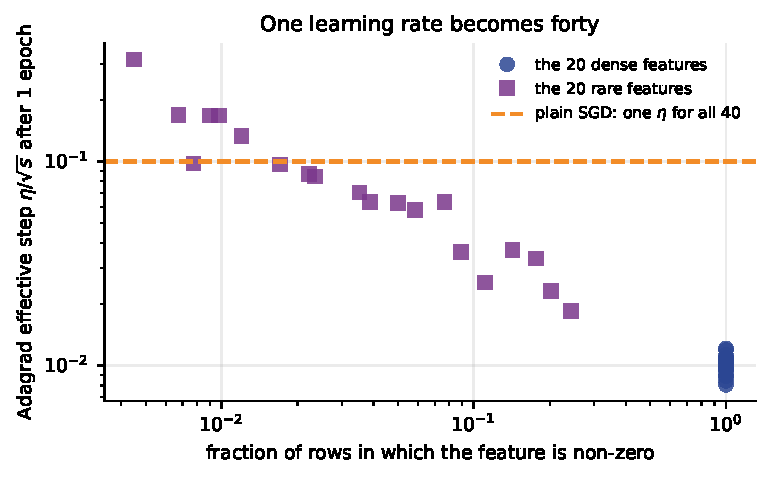
\includegraphics[width=\textwidth]{perparam.pdf}
    \end{column}
    \begin{column}{0.42\textwidth}
      \begin{block}{After one epoch, $\eta = 0.10$}
        \small
        \begin{tabular}{@{}lr@{}}
          dense features & $0.00996$\\
          rarest feature & $0.3165$\\
          \midrule
          spread across the 40 & $39.3\times$\\
        \end{tabular}
      \end{block}
      \begin{exampleblock}{The whole point}
        \small You supplied \emph{one} number. Adagrad turned it into forty, and
        gave the rarest feature a step $32\times$ larger than the dense ones ---
        because it has $32\times$ less evidence about it.
      \end{exampleblock}
    \end{column}
  \end{columns}
\end{frame}

\begin{frame}[fragile]{Does it actually learn the rare features?}
Same sparse problem, ten epochs, $B = 32$, each optimiser at its own best
$\eta$:
\begin{outblk}
sgd      eta=0.01   MSE 0.0853   dense 1.0004   5 rarest 0.1562
adagrad  eta=0.10   MSE 0.0105   dense 0.9999   5 rarest 0.8631
\end{outblk}
\onslide<2->
\begin{center}\small
  $0.156 \rightarrow 0.863$ on the rare features, and the dense ones are
  \emph{still} recovered exactly. The MSE fell by a factor of eight.
\end{center}
\onslide<3->
\begin{alertblock}{This is the case Adagrad was built for}
  \footnotesize Sparse features are the normal situation in text, in recommender
  systems, and in anything one-hot encoded. If your feature matrix is mostly
  zeros, try Adagrad before you try anything clever.
\end{alertblock}
\end{frame}

\begin{frame}[fragile]{The flaw: the sum only ever grows}
$s_t = \sum_{k\le t} g_k^2$ cannot decrease --- not even at the optimum, where
mini-batch gradients are still non-zero.
\begin{lstlisting}
st["s"] += g*g                        # Adagrad on load_diabetes, eta=0.05
w = w - eta*g/(np.sqrt(st["s"]) + 1e-8)
\end{lstlisting}
\begin{outblk}
update     1   s =    1.667   effective step = 0.03873
update   100   s =   11.477   effective step = 0.01476
update  1000   s =   58.171   effective step = 0.00656
update  2800   s =  148.007   effective step = 0.00411
after 200 epochs                   MSE 0.4845
\end{outblk}
\onslide<2->
\begin{alertblock}{The learning rate you set is not the one you get}
  \footnotesize By update $2800$ the effective step is $9.4\times$ smaller and
  still falling like $1/\sqrt{t}$. Convex problems converge anyway; a deep
  network \textbf{stalls}.
\end{alertblock}
\end{frame}

\begin{frame}[shrink=8]{Drawn: growth without bound}
  \begin{center}
    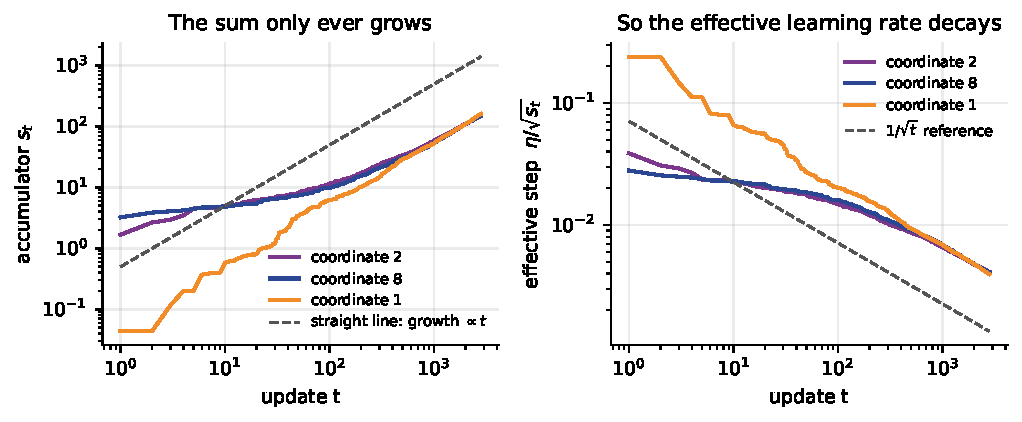
\includegraphics[width=0.88\textwidth]{adagrad_accum.pdf}
  \end{center}
  \begin{center}\small
    Left: three coordinates' accumulators, log--log, against a straight line of
    slope $1$. The sum grows \textbf{linearly in $t$}. Right: therefore the
    effective step decays as $1/\sqrt{t}$ --- a learning-rate schedule you never
    asked for and cannot switch off.
  \end{center}
\end{frame}

\begin{frame}[fragile,shrink=6]{Predict first \#2}
A noisy one-dimensional bowl. Minimum at $w = 50$, start at $w = 0$, gradient
noise of standard deviation $20$ that never dies away. $\eta = 0.5$ for both.

\begin{center}
  \textbf{After 20{,}000 updates, where has Adagrad got to?
  And where is RMSprop after only 100?}
\end{center}
\vspace{0.3em}
\onslide<2->
\begin{outblk}
adagrad  t=100   w=  9.01 step=0.00055  t=1000  w= 26.50 step=0.00023
         t=5000  w= 44.80 step=0.00017  t=20000 w= 50.05 step=0.00013
rmsprop  t=100   w= 44.49 step=0.01784  t=1000  w= 50.63 step=0.02488
         t=5000  w= 53.46 step=0.02873  t=20000 w= 48.60 step=0.02334
the minimum is at w = 50
\end{outblk}
\onslide<3->
\begin{alertblock}{Adagrad needs 4{,}874 updates to reach RMSprop's 100th}
  \footnotesize It does arrive eventually --- $50.05$ is a good answer. But its
  step has collapsed to $1.3\times10^{-4}$ getting there. Move the minimum now
  and it will never follow. Note RMSprop's own row wanders --- $50.63$, $53.46$,
  $48.60$ --- because its step never shrank either. That is coming.
\end{alertblock}
\end{frame}

% =====================================================================
\section{RMSprop}
\label{sec:rmsprop}

\begin{frame}[shrink=12]{RMSprop: one symbol changes}
  \begin{columns}[T]
    \begin{column}{0.46\textwidth}
      \begin{block}{Adagrad}
        \centering
        $s_t = s_{t-1} + g_t^2$\\[0.3em]
        {\small a \textbf{sum} --- unbounded}
      \end{block}
    \end{column}
    \begin{column}{0.5\textwidth}
      \begin{exampleblock}{RMSprop}
        \centering
        $s_t = \gamma\, s_{t-1} + (1-\gamma)\, g_t^2$\\[0.3em]
        {\small an \textbf{average} --- bounded}
      \end{exampleblock}
    \end{column}
  \end{columns}
  \vspace{0.6em}
  \begin{center}
    $w \leftarrow w - \dfrac{\eta}{\sqrt{s_t}+\varepsilon}\odot g_t$
    \qquad unchanged. \quad $\gamma = 0.9$ by default.
  \end{center}
  \vspace{0.5em}
  \begin{alertblock}{The same exponentially weighted average as momentum}
    Weight $\gamma^j$ on the gradient $j$ steps ago; total weight $1$; memory
    about $1/(1-\gamma) = 10$ steps. Here it averages $g^2$, not $g$.
  \end{alertblock}
  \vspace{0.2em}
  \begin{center}\small
    Hinton, Coursera lecture 6e, 2012 --- famously never published as a paper.
  \end{center}
\end{frame}

\begin{frame}[shrink=8]{By hand: three steps of RMSprop}
  Same bowl, same $\eta = 0.5$, now with $\gamma = 0.9$.
  \begin{center}\small
  \begin{tabular}{@{}rrrrrr@{}}
    \toprule
    $t$ & $g_t$ & $s_t = 0.9 s_{t-1}+0.1 g_t^2$ & $\sqrt{s_t}$
        & step & $w_t$\\
    \midrule
    1 & $-6.0000$ & $3.6000$ & $1.8974$ & $-1.5811$ & $1.5811$\\
    2 & $-2.8377$ & $4.0453$ & $2.0113$ & $-0.7055$ & $2.2866$\\
    3 & $-1.4268$ & $3.8443$ & $1.9607$ & $-0.3639$ & $2.6504$\\
    \bottomrule
  \end{tabular}
  \end{center}
  \vspace{0.2em}
  \begin{alertblock}{Adagrad reached $1.064$; RMSprop reached $2.650$}
    \small Identical $\eta$, identical bowl, target $3$. Look at row 3: Adagrad's
    denominator was $8.94$ and climbing, RMSprop's was $1.96$ and it \emph{fell}
    from $2.01$. An average can go down.
  \end{alertblock}
  \vspace{0.2em}
  \begin{center}\small
    Why the first step is $3.16\eta$ and not $\eta$: $s_1 = (1-\gamma)g_1^2$, so
    $\sqrt{s_1} = \sqrt{0.1}\,|g_1|$ and the step is $\eta/\sqrt{1-\gamma}$.
  \end{center}
\end{frame}

\begin{frame}[fragile]{The same thing in code}
\begin{lstlisting}
eta, gamma = 0.5, 0.9
w, s = 0.0, 0.0
for t in (1, 2, 3):
    g = 2.0*(w - 3.0)
    s = gamma*s + (1 - gamma)*g*g            # the only changed line
    w = w - eta*g/(np.sqrt(s) + 1e-8)
\end{lstlisting}
\begin{outblk}
t=1  g= -6.0000  s=  3.6000  sqrt(s)= 1.8974  step= -1.5811  w=1.5811
t=2  g= -2.8377  s=  4.0453  sqrt(s)= 2.0113  step= -0.7055  w=2.2866
t=3  g= -1.4268  s=  3.8443  sqrt(s)= 1.9607  step= -0.3639  w=2.6504
\end{outblk}
\begin{center}\small
  Diff against the Adagrad listing: \texttt{s = s + g*g} became
  \texttt{s = gamma*s + (1-gamma)*g*g}. That is the whole of RMSprop.
\end{center}
\end{frame}

\begin{frame}[shrink=10]{Two denominators, drawn}
  \begin{center}
    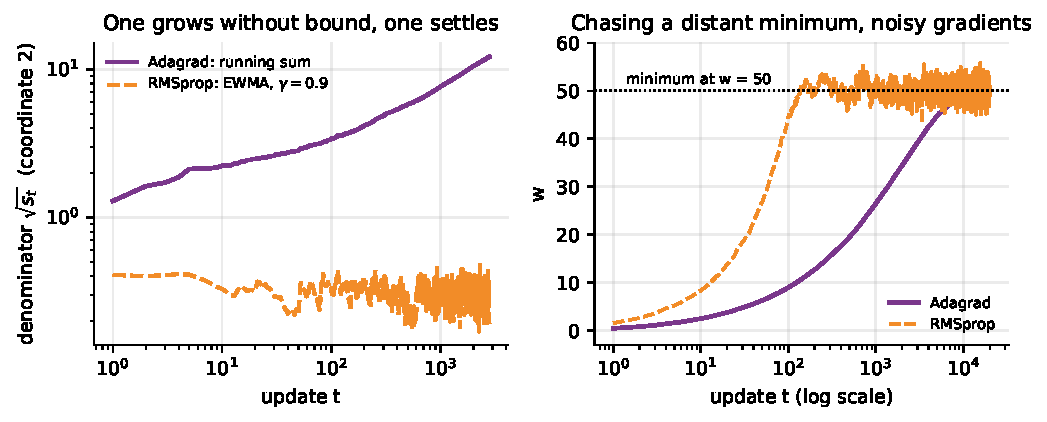
\includegraphics[width=0.86\textwidth]{adagrad_vs_rms.pdf}
  \end{center}
  \begin{columns}[T]
    \begin{column}{0.47\textwidth}
      \begin{block}{Measured, coordinate 2, 2800 updates}
        \small Adagrad's $\sqrt{s}$: $1.29 \rightarrow 12.17$.\\
        RMSprop's: $0.41 \rightarrow 0.19$.
      \end{block}
    \end{column}
    \begin{column}{0.49\textwidth}
      \begin{alertblock}{What RMSprop gives up}
        \small Adagrad has a convergence proof on convex problems; RMSprop has
        none, and it does \emph{not} settle --- it hovers in a noise band whose
        width is set by $\eta$, exactly like constant-step SGD.
      \end{alertblock}
    \end{column}
  \end{columns}
\end{frame}

% =====================================================================
\section{Adadelta}
\label{sec:adadelta}

\begin{frame}[shrink=6]{Adadelta: the units are wrong}
  Do a dimensional analysis of the update. Write $[w]$ for the units of a
  parameter and $[J]$ for the units of the loss, so $g$ has units $[J]/[w]$.
  \begin{center}\small
  \begin{tabular}{@{}llc@{}}
    \toprule
    \textbf{Method} & \textbf{Update} & \textbf{Units}\\
    \midrule
    SGD              & $-\eta g$          & $[\eta]\,[J]/[w]$\\[2pt]
    Adagrad, RMSprop & $-\eta g/\sqrt{s}$ & $[\eta]$ \quad{\small($\sqrt{s}$ cancels $g$)}\\[2pt]
    Newton           & $-H^{-1}g$         & $[w]$ \quad{\small(correct --- but $H$ is unaffordable)}\\
    \bottomrule
  \end{tabular}
  \end{center}
  \vspace{0.4em}
  \begin{exampleblock}{Zeiler's observation (2012)}
    Adagrad and RMSprop have already cancelled the gradient's units. All that is
    missing is a quantity carrying the units of $w$ --- and we have one lying
    around: \textbf{the size of the recent updates themselves}.
  \end{exampleblock}
  \vspace{0.3em}
  \begin{center}\Large
    $\Delta w_t = -\dfrac{\mathrm{RMS}[\Delta w]_{t-1}}{\mathrm{RMS}[g]_t}\, g_t$
    \qquad {\normalsize no $\eta$ anywhere}
  \end{center}
\end{frame}

\begin{frame}[shrink=6]{Adadelta in full: two accumulators, no learning rate}
  \begin{center}
  \begin{tabular}{@{}ll@{}}
    \toprule
    gradient accumulator & $s_t = \rho\, s_{t-1} + (1-\rho)\, g_t^2$\\[3pt]
    the step             & $\Delta w_t = -\dfrac{\sqrt{d_{t-1}+\varepsilon}}
                            {\sqrt{s_t+\varepsilon}}\; g_t$\\[8pt]
    update accumulator   & $d_t = \rho\, d_{t-1} + (1-\rho)\, \Delta w_t^2$\\[3pt]
    parameters           & $w \leftarrow w + \Delta w_t$\\
    \bottomrule
  \end{tabular}
  \end{center}
  \vspace{0.6em}
  \begin{columns}[T]
    \begin{column}{0.48\textwidth}
      \begin{block}{Defaults}
        $\rho = 0.9$, \; $\varepsilon = 10^{-6}$. Note $\varepsilon$ sits
        \textbf{inside} both square roots here, and it is far larger than
        Adagrad's $10^{-8}$.
      \end{block}
    \end{column}
    \begin{column}{0.48\textwidth}
      \begin{alertblock}{Where does the first step come from?}
        $d_0 = 0$, so $\mathrm{RMS}[\Delta w]_0 = \sqrt{\varepsilon} = 10^{-3}$.
        The algorithm \textbf{bootstraps itself out of $\varepsilon$}.
      \end{alertblock}
    \end{column}
  \end{columns}
\end{frame}

\begin{frame}[fragile]{By hand and in code: Adadelta creeps, then speeds up}
Same bowl $f(w)=(w-3)^2$, $\rho = 0.9$, $\varepsilon = 10^{-6}$, $w_0 = 0$.
\begin{lstlisting}
s    = rho*s + (1 - rho)*g*g
dw   = -np.sqrt(dacc + epsd)/np.sqrt(s + epsd) * g
dacc = rho*dacc + (1 - rho)*dw*dw
\end{lstlisting}
\begin{outblk}
  t        g   RMS[g]_t  RMS[dw]_{t-1}         dw          w
  1  -6.0000     1.8974       0.001000   0.003162   0.003162
  2  -5.9937     2.6139       0.001414   0.003243   0.006405
  3  -5.9872     3.1199       0.001718   0.003297   0.009702
 10  -5.9397     4.8137       0.002825   0.003485   0.033635
200  -4.3511     4.4339       0.004662   0.004575   0.829020
\end{outblk}
\onslide<2->
\begin{center}\small
  Check row 1 by hand: $\sqrt{10^{-6}}\times 6 / 1.8974 = 0.003162$;
  after 200 steps $w = 0.83$.\\
  \textbf{Adadelta buys freedom from $\eta$ with a slow start.}
\end{center}
\end{frame}

\begin{frame}[fragile,shrink=8]{It works out its own step size}
On \texttt{load\_diabetes}. The ratio
$r_t = \mathrm{RMS}[\Delta w]_{t-1}/\mathrm{RMS}[g]_t$ \emph{is} a step size,
so it is directly comparable with an $\eta$.
\begin{outblk}
Adadelta's own step size  r_t = RMS[dw]_{t-1} / RMS[g]_t  (coordinate 2)
   update     1    r = 0.002449
   update   100    r = 0.005168
   update  2800    r = 0.012292
   the eta a human found by search for plain SGD  0.005000
\end{outblk}
\onslide<2->
\begin{center}
  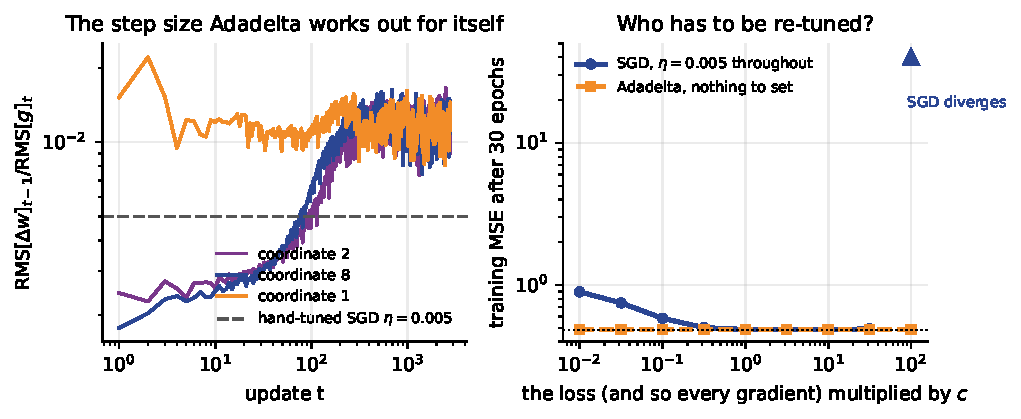
\includegraphics[width=0.90\textwidth]{adadelta.pdf}
\end{center}
\end{frame}

\begin{frame}[fragile,shrink=4]{Predict first \#3}
Multiply the loss by a constant $c$. Every gradient is multiplied by $c$ too;
nothing else changes, and \emph{the optimum is in exactly the same place}.

\begin{center}
  \textbf{SGD keeps $\eta = 0.005$ and Adadelta keeps nothing. Who survives
  $c = 0.01$? Who survives $c = 100$?}
\end{center}
\vspace{0.3em}
\onslide<2->
\begin{outblk}
multiply the loss by c; nothing else changes.  30 epochs, B=32
c           SGD eta=0.005       Adadelta
0.01               0.8941         0.4860
1                  0.4860         0.4859
100              diverged         0.4859
least-squares optimum                     0.4823
\end{outblk}
\onslide<3->
\begin{alertblock}{Adadelta varies by a factor of $1.0002$ over four decades}
  \footnotesize That is what ``dimensionally consistent'' buys you. A learning
  rate is a number in units of $[w]^2/[J]$; change the units of $J$ and it is
  wrong. Adadelta's step carries the units of $w$, so nothing to re-tune.
\end{alertblock}
\end{frame}

\begin{frame}[fragile]{Adadelta on the real problem}
\texttt{load\_diabetes}, mini-batch $B=32$, and \textbf{no learning rate
supplied}:
\begin{outblk}
Adadelta, no learning rate,  5 epochs   MSE 0.5665
Adadelta, no learning rate, 30 epochs   MSE 0.4859
least-squares optimum                    MSE 0.4823
\end{outblk}
\onslide<2->
\begin{columns}[T]
  \begin{column}{0.48\textwidth}
    \begin{exampleblock}{It gets there}
      \small $0.4859$ against an optimum of $0.4823$ --- as good as tuned SGD
      ($0.4860$), with nothing to tune.
    \end{exampleblock}
  \end{column}
  \begin{column}{0.48\textwidth}
    \begin{alertblock}{It gets there last}
      \small At 5 epochs it is at $0.5665$, the worst of the six optimisers we
      are about to compare. The slow start is real.
    \end{alertblock}
  \end{column}
\end{columns}
\onslide<3->
\begin{center}\small
  PyTorch's \texttt{Adadelta} still takes an \texttt{lr}, defaulting to $1.0$:
  a pure multiplier on $\Delta w$, not a step size.
\end{center}
\end{frame}

% =====================================================================
\section{Adam}
\label{sec:adam}

\begin{frame}[shrink=10]{Adam: momentum $+$ RMSprop, both as averages}
  \begin{center}
  \begin{tabular}{@{}ll@{}}
    \toprule
    first moment (direction) & $m_t = \beta_1 m_{t-1} + (1-\beta_1)\, g_t$
      \hfill{\small from momentum}\\[3pt]
    second moment (scale)    & $v_t = \beta_2 v_{t-1} + (1-\beta_2)\, g_t^2$
      \hfill{\small from RMSprop}\\[6pt]
    bias correction          & $\hat m_t = \dfrac{m_t}{1-\beta_1^{\,t}}$,
      \qquad $\hat v_t = \dfrac{v_t}{1-\beta_2^{\,t}}$\\[8pt]
    the step                 & $w \leftarrow w - \dfrac{\eta\, \hat m_t}
                                {\sqrt{\hat v_t}+\varepsilon}$\\
    \bottomrule
  \end{tabular}
  \end{center}
  \vspace{0.5em}
  \begin{center}\small
    Defaults: $\beta_1 = 0.9$, $\beta_2 = 0.999$, $\varepsilon = 10^{-8}$,
    $\eta = 0.001$. Kingma and Ba, ICLR 2015.
  \end{center}
  \vspace{0.3em}
  \begin{alertblock}{Note the $(1-\beta)$ convention}
    Both moments are \textbf{true} running averages --- the second of the two
    momentum conventions, not $v \leftarrow \beta v + g$. That is exactly why a
    bias-correction line is needed at all.
  \end{alertblock}
\end{frame}

\begin{frame}[shrink=6]{Why the first step is biased}
  Start with $m_0 = v_0 = 0$ and unroll one step:
  \begin{align*}
    m_1 &= (1-\beta_1)\,g_1 = 0.1\, g_1, &
    v_1 &= (1-\beta_2)\, g_1^2 = 0.001\, g_1^2 .
  \end{align*}
  \begin{center}
    Both are pulled towards \textbf{zero} --- $m_1$ is one tenth of the size it
    should be, $v_1$ one thousandth.
  \end{center}
  \vspace{0.4em}
  \begin{exampleblock}{After $t$ steps of a constant gradient $g$}
    \centering
    $m_t = (1-\beta_1^{\,t})\, g$ \qquad so \qquad
    $\hat m_t = \dfrac{m_t}{1-\beta_1^{\,t}} = g$. \quad Unbiased, by
    construction.
  \end{exampleblock}
  \vspace{0.4em}
  \begin{alertblock}{The mismatch is the problem, not the shrinkage}
    \small $m$ shrinks by $10$; $\sqrt{v}$ shrinks by $\sqrt{1000} = 31.6$. They
    do \emph{not} cancel, and the ratio $m/\sqrt{v}$ comes out $31.6/10 = 3.16$
    times \textbf{too large}.
  \end{alertblock}
\end{frame}

\begin{frame}[shrink=5]{By hand: Adam, step 1}
  $f(w)=(w-3)^2$, $\eta = 0.1$, $\beta_1 = 0.9$, $\beta_2 = 0.999$, $w_0 = 0$,
  $m_0 = v_0 = 0$.
  \begin{center}\small
  \begin{tabular}{@{}ll@{}}
    \toprule
    gradient      & $g_1 = 2(0 - 3) = -6$\\[3pt]
    first moment  & $m_1 = 0.9(0) + 0.1(-6) = -0.6$\\[3pt]
    second moment & $v_1 = 0.999(0) + 0.001(36) = 0.036$\\[3pt]
    correct $m$   & $\hat m_1 = -0.6/(1-0.9) = -0.6/0.1 = -6$\\[3pt]
    correct $v$   & $\hat v_1 = 0.036/(1-0.999) = 0.036/0.001 = 36$\\[3pt]
    denominator   & $\sqrt{\hat v_1} = 6$\\[3pt]
    step          & $\Delta w = -0.1 \times (-6)/6 = +0.1$\\[3pt]
    \textbf{new parameter} & $\mathbf{w_1 = 0.1}$\\
    \bottomrule
  \end{tabular}
  \end{center}
  \vspace{0.2em}
  \begin{exampleblock}{$\hat m_1 = g_1$ and $\hat v_1 = g_1^2$, exactly}
    \small So the corrected first step is $-\eta\, g_1/\lvert g_1\rvert =
    \pm\eta$. \textbf{Adam's first step has size exactly $\eta$, downhill,
    whatever the gradient's magnitude.}
  \end{exampleblock}
\end{frame}

\begin{frame}[fragile]{Predict first \#4}
Same step, but delete the two bias-correction lines: use $m_1$ and $v_1$ raw.
\begin{center}
  \textbf{The corrected first step was $+0.1000$. What is the uncorrected one,
  and by what factor is it wrong?}
\end{center}
\onslide<2->
\begin{outblk}
first gradient                g1        = -6.0000
uncorrected  m1 / sqrt(v1)              = -3.1623
corrected    mhat1 / sqrt(vhat1)        = -1.0000
ratio  (1-b1)/sqrt(1-b2)                = 3.1623
worst overshoot at t=12, factor 6.57 too big
within 1% of the corrected step only from t=3916
\end{outblk}
\onslide<3->
\begin{alertblock}{Three times too big at $t=1$, six and a half times at $t=12$}
  \footnotesize The two corrections fade at very different rates: $\beta_1$'s is
  within $1\%$ of $1$ by step $44$, $\beta_2$'s only by step \textbf{4613}. That
  gap is the reason bias correction exists.
\end{alertblock}
\end{frame}

\begin{frame}[shrink=8]{Bias correction, drawn}
  \begin{center}
    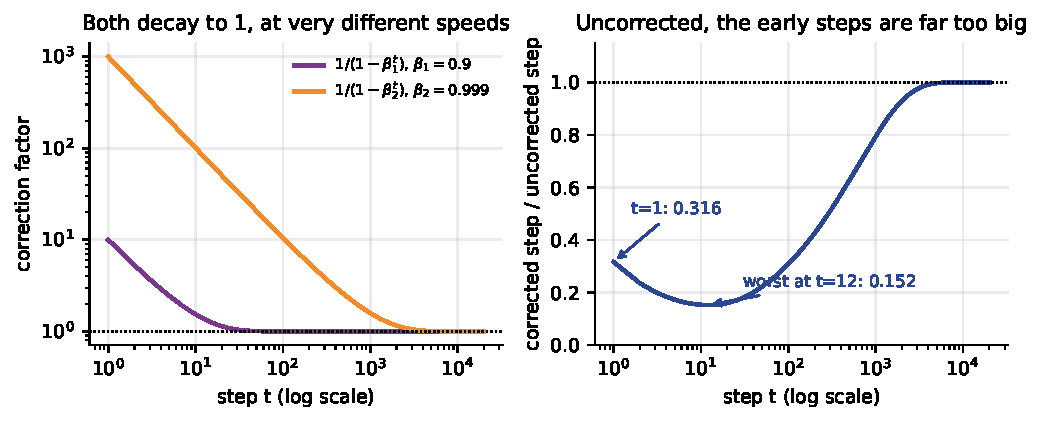
\includegraphics[width=0.88\textwidth]{adam_bias.pdf}
  \end{center}
  \begin{center}\small
    Left: the two correction factors $1/(1-\beta_1^t)$ and $1/(1-\beta_2^t)$,
    log--log --- one decays in tens of steps, the other in thousands. Right:
    their combined effect. The uncorrected step is \textbf{$3.16\times$ too big
    at $t=1$}, worst at $t=12$ at \textbf{$6.57\times$}, and within one per cent
    only after $t = 3916$.
  \end{center}
\end{frame}

\begin{frame}[fragile,shrink=10]{The two trajectories, run side by side}
Both runs are Adam on $f(w)=(w-3)^2$ from $w_0=0$ with $\eta = 0.1$. The only
difference is the two correction lines.
\begin{outblk}
               t=1       t=2       t=3       t=12
w, corrected   0.1000    0.1999    0.2996    1.1753
w, no bc       0.3162    0.7393    1.2263    4.4123
step size, corrected: never exceeds 0.1000  (you asked for 0.1)
step size, no bc:     peaks at      0.5340  = 5.3 times too big
furthest past the minimum, corrected  3.1773 at t=53
furthest past the minimum, no bc      4.4123 at t=12
\end{outblk}
\onslide<2->
\begin{center}
  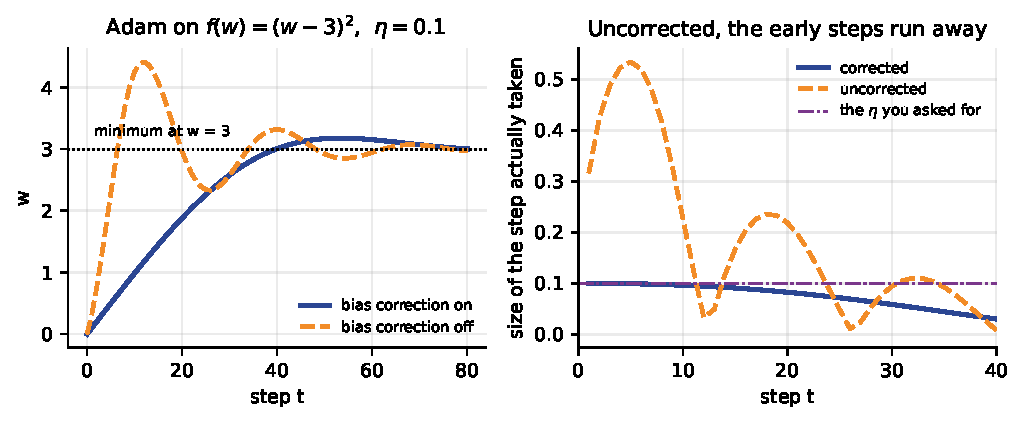
\includegraphics[width=0.74\textwidth]{adam_traj.pdf}
\end{center}
\end{frame}

\begin{frame}[shrink=7]{By hand: Adam, steps 2 and 3}
  Carrying $w_1 = 0.1$, $m_1 = -0.6$, $v_1 = 0.036$ forward.
  \begin{center}\small
  \begin{tabular}{@{}rrrrrrr@{}}
    \toprule
    $t$ & $g_t$ & $m_t$ & $v_t$ & $\hat m_t$ & $\sqrt{\hat v_t}$ & $w_t$\\
    \midrule
    1 & $-6.0000$ & $-0.60000$ & $0.036000$ & $-6.0000$ & $6.0000$ & $0.100000$\\
    2 & $-5.8000$ & $-1.12000$ & $0.069604$ & $-5.8947$ & $5.9008$ & $0.199897$\\
    3 & $-5.6002$ & $-1.56802$ & $0.100897$ & $-5.7861$ & $5.8022$ & $0.299618$\\
    \bottomrule
  \end{tabular}
  \end{center}
  \vspace{0.2em}
  Row 2 in full: $m_2 = 0.9(-0.6) + 0.1(-5.8) = -1.12$;\;
  $\hat m_2 = -1.12/(1-0.81) = -5.8947$;\;
  $\hat v_2 = 0.069604/(1-0.998001) = 34.819$.
  \vspace{0.2em}
  \begin{alertblock}{Every step is almost exactly $\eta = 0.1$}
    \small $0.1000,\ 0.0999,\ 0.0997$. The ratio $\hat m/\sqrt{\hat v}$ stays
    near $\pm1$ because both moments track the \emph{same} gradient sequence.
    \textbf{Adam moves at a speed you set, not one the gradient sets.}
  \end{alertblock}
\end{frame}

\begin{frame}[fragile,shrink=3]{The same thing in code}
\begin{lstlisting}
eta, b1, b2, eps = 0.1, 0.9, 0.999, 1e-8
w, m, v = 0.0, 0.0, 0.0
for t in (1, 2, 3):
    g = 2.0*(w - 3.0)
    m = b1*m + (1 - b1)*g
    v = b2*v + (1 - b2)*g*g
    mh, vh = m/(1 - b1**t), v/(1 - b2**t)         # bias correction
    w = w - eta*mh/(np.sqrt(vh) + eps)
\end{lstlisting}
\begin{outblk}
  t         g          m          v       mhat  sqrt(vhat)          w
  1   -6.0000   -0.60000   0.036000    -6.0000      6.0000   0.100000
  2   -5.8000   -1.12000   0.069604    -5.8947      5.9008   0.199897
  3   -5.6002   -1.56802   0.100897    -5.7861      5.8022   0.299618
\end{outblk}
\begin{center}\small
  Six lines. Adam is Adagrad's idea, RMSprop's fix, momentum's direction, and
  two divisions.
\end{center}
\end{frame}

\begin{frame}[fragile]{Does bias correction matter in practice?}
\texttt{load\_diabetes}, $\eta = 0.02$, $B = 32$, with and without the two
correction lines:
\begin{outblk}
Adam, eta=0.02, B=32          epoch 1   epoch 5   epoch 30
bias correction on              0.5369    0.4888     0.4929
bias correction off             0.5758    0.4885     0.4960
\end{outblk}
\onslide<2->
\begin{columns}[T]
  \begin{column}{0.5\textwidth}
    \begin{block}{The damage is early, then gone}
      \small $0.5369$ against $0.5758$ at epoch~1; indistinguishable by
      epoch~5. On a two-minute convex run: invisible.
    \end{block}
  \end{column}
  \begin{column}{0.46\textwidth}
    \begin{alertblock}{So why does it exist?}
      \small Because on a large model those first hundred oversized steps land
      you somewhere you cannot recover from --- and because $\eta$ tuned
      \emph{with} correction is not $\eta$ tuned without it.
    \end{alertblock}
  \end{column}
\end{columns}
\onslide<3->
\begin{center}\small
  \textbf{Warmup} --- ramping $\eta$ up over the first few thousand steps --- is
  the modern belt-and-braces version of the same idea.
\end{center}
\end{frame}

% =====================================================================
\section[Practice]{Numerical practice}
\label{sec:practice}

\begin{frame}[fragile]{Six optimisers, one problem}
\texttt{load\_diabetes}, $B=32$, 30 epochs, each at its own tuned $\eta$:
\begin{outblk}
optimiser     eta    epoch 1  epoch 5 epoch 30
sgd         0.005     0.7393   0.5358   0.4860
momentum    0.005     0.5711   0.4870   0.4846
adagrad     0.050     0.5349   0.4884   0.4859
rmsprop     0.005     0.6613   0.4948   0.4853
adadelta    1.000     0.8157   0.5665   0.4859
adam        0.020     0.5369   0.4888   0.4929
optimum                                 0.4823
\end{outblk}
\onslide<2->
\begin{alertblock}{Read the last column before the first}
  \footnotesize Every one of them lands between $0.4846$ and $0.4929$. On a
  well-conditioned convex problem with a tuned $\eta$, \textbf{the choice of
  optimiser is worth about one per cent} --- and Adam is the \emph{worst} at
  epoch 30, because it never settles.
\end{alertblock}
\end{frame}

\begin{frame}[shrink=8]{The same six, drawn}
  \begin{center}
    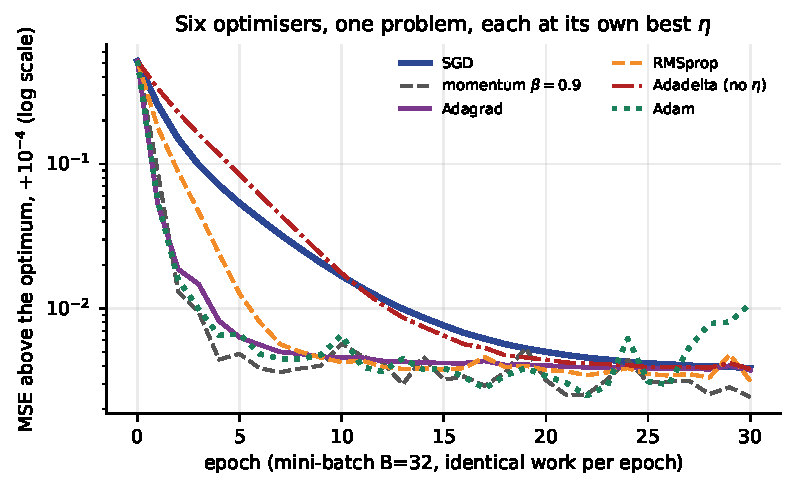
\includegraphics[width=0.60\textwidth]{optimcompare.pdf}
  \end{center}
  \begin{center}\small
    Distance above the optimum, log scale. The adaptive methods win the first
    two epochs and then flatten into a noise band; momentum quietly keeps
    descending. \textbf{If you read only the first epoch you would draw the
    opposite conclusion from the right one.}
  \end{center}
\end{frame}

\begin{frame}[fragile]{And the sparse problem, all five}
The same forty-feature problem from the start of the lecture, ten epochs:
\begin{outblk}
optimiser     eta        MSE     dense  5 rarest
sgd         0.010     0.0853    1.0004   0.1562
momentum    0.001     0.0853    0.9998   0.1557
adagrad     0.100     0.0105    0.9999   0.8631
rmsprop     0.005     0.0106    1.0003   0.9846
adam        0.050     0.0125    0.9990   1.0051
\end{outblk}
\onslide<2->
\begin{alertblock}{Here the choice of optimiser is worth a factor of eight}
  \footnotesize Momentum does not help at all --- it averages the direction, not
  the scale, so a rare feature's rare gradient stays rare. Every
  \emph{per-coordinate} method fixes it. \textbf{Sparse data is where adaptive
  methods earn their keep.}
\end{alertblock}
\end{frame}

\begin{frame}[fragile,shrink=4]{Predict first, one last time}
A grid of 25 learning rates from $10^{-4}$ to $3$. For each optimiser, count how
many of them land within 5\% of the optimum in 10 epochs.

\begin{center}
  \textbf{Which optimiser tolerates the widest range of $\eta$ --- and how many
  decades wide is that range?}
\end{center}
\vspace{0.3em}
\onslide<2->
\begin{outblk}
sgd         8/25 grid points work:  0.0048 to 0.0965  (1.31 decades)
momentum   10/25 grid points work:  0.0006 to 0.0266  (1.68 decades)
adagrad    13/25 grid points work:  0.0173 to 3.0000  (2.24 decades)
rmsprop     9/25 grid points work:  0.0020 to 0.0628  (1.49 decades)
adam        9/25 grid points work:  0.0031 to 0.0965  (1.49 decades)
\end{outblk}
\onslide<3->
\begin{alertblock}{Adagrad --- still working at the top of the grid}
  \footnotesize Its own $1/\sqrt{t}$ decay rescues an $\eta$ that would destroy
  every other method; $3.0$ is where we stopped looking, not where it failed.
  \textbf{This, not final accuracy, is what adaptive optimisers actually buy: a
  wider target to aim at.}
\end{alertblock}
\end{frame}

\begin{frame}[shrink=8]{The window of usable learning rates, drawn}
  \begin{center}
    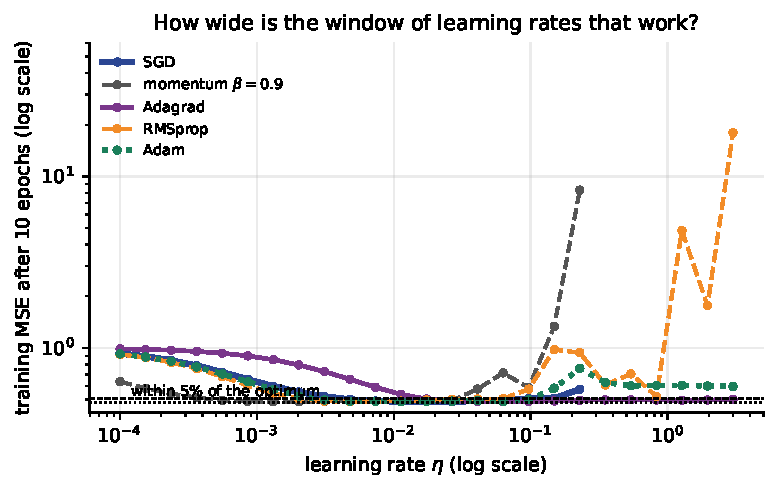
\includegraphics[width=0.60\textwidth]{lrsensitivity.pdf}
  \end{center}
  \begin{center}\small
    Every curve is a bathtub with a hard right-hand wall: below the wall a run
    is merely slow, above it the run is destroyed. Adagrad's bathtub is $2.24$
    decades wide, plain SGD's is $1.31$.
  \end{center}
\end{frame}

\begin{frame}[fragile,shrink=6]{Back to the ravine}
$f(w) = 0.01w_1^2 + 2w_2^2$, $\kappa = 200$, start at $(9, 1)$:
\begin{outblk}
optimiser      eta   iters to ||w||<1e-3  ||w|| after 1200
gd           0.475                   954          9.99e-04
momentum     0.475                   135          7.88e-04
adagrad      0.500                   805          9.97e-04
rmsprop      0.050                 never          3.54e-02
adam         0.100                   262          9.89e-04
\end{outblk}
\onslide<2->
\begin{columns}[T]
  \begin{column}{0.42\textwidth}
    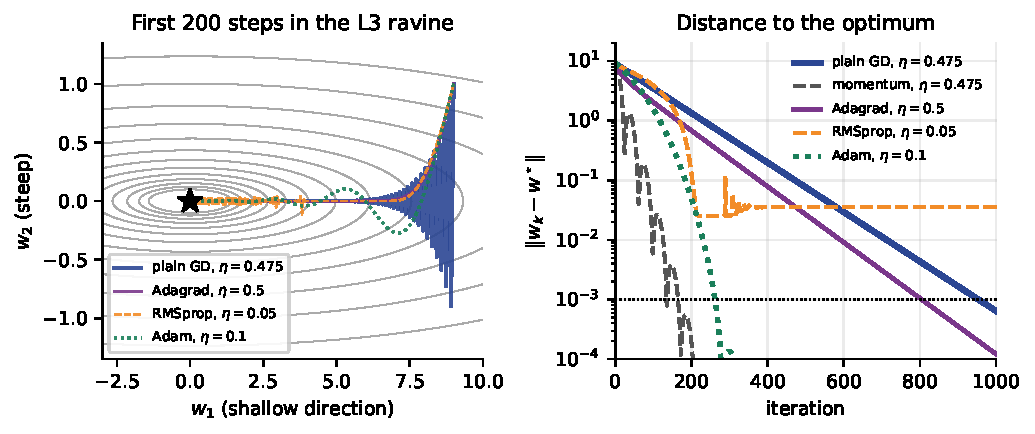
\includegraphics[width=\textwidth]{ravine_adaptive.pdf}
  \end{column}
  \begin{column}{0.55\textwidth}
    \begin{alertblock}{Momentum still wins here}
      \footnotesize A ravine is a \emph{curvature} problem, and adaptive methods
      measure \emph{gradients}. Momentum's $\sqrt{\kappa}$ acceleration is the
      right tool: $135$ beats everything.
    \end{alertblock}
    \begin{block}{RMSprop never arrives}
      \footnotesize Constant $\eta$, bounded denominator: a limit cycle at
      $3.5\times 10^{-2}$.
    \end{block}
  \end{column}
\end{columns}
\end{frame}

\begin{frame}[fragile]{Two numerical details that will cost you a run}
\begin{outblk}
RMSprop, epsilon =   1e-08   MSE after 10 epochs 0.4864
RMSprop, epsilon =   1e-06   MSE after 10 epochs 0.4864
RMSprop, epsilon =   1e-04   MSE after 10 epochs 0.4864
RMSprop, epsilon =   1e-02   MSE after 10 epochs 0.4864
RMSprop, epsilon =   1e-01   MSE after 10 epochs 0.4870
RMSprop, epsilon =   1e+00   MSE after 10 epochs 0.5185
\end{outblk}
\onslide<2->
\begin{outblk}
Adam, decay off  epoch  5   MSE 0.4888    epoch 30   MSE 0.4929
Adam, decay on   epoch  5   MSE 0.4877    epoch 30   MSE 0.4850
\end{outblk}
\onslide<3->
\begin{center}\small
  \textbf{$\varepsilon$ is not a hyperparameter until it is.} Anything below
  $10^{-2}$ is identical here; at $\varepsilon = 1$ it dominates $\sqrt{s}$ and
  RMSprop degenerates into plain SGD.\\[0.3em]
  \textbf{Adam got worse between epoch 5 and epoch 30}
  ($0.4888 \to 0.4929$). A $1/(1+ct)$ decay fixes it: $0.4850$. Adaptive does
  not mean schedule-free.
\end{center}
\end{frame}

\begin{frame}[shrink=7]{Which one should you use?}
  \begin{center}\small
  \begin{tabular}{@{}lp{4.2cm}p{4.6cm}@{}}
    \toprule
    & \textbf{Reach for it when} & \textbf{Watch out for}\\
    \midrule
    SGD $+$ momentum & you can afford to tune and you want the best final
      number & narrowest usable $\eta$ window ($1.31$ decades)\\[3pt]
    Adagrad & the features are \textbf{sparse}; short runs & the step decays as
      $1/\sqrt{t}$ and stalls\\[3pt]
    RMSprop & non-stationary objectives; recurrent nets & no convergence
      guarantee; hovers\\[3pt]
    Adadelta & you have no time to tune anything & slowest start of the six\\[3pt]
    \textbf{Adam} & \textbf{the default}: anything new, first attempt & does not
      settle; decay $\eta$ at the end\\
    \bottomrule
  \end{tabular}
  \end{center}
  \vspace{0.3em}
  \begin{exampleblock}{The honest recipe}
    \small \textbf{Standardise. Start with Adam at $\eta = 10^{-3}$ and
    $B = 32$.} If the result matters, tune SGD${}+{}$momentum against it --- on
    our data it won, $0.4846$ against $0.4929$.
  \end{exampleblock}
\end{frame}

% =====================================================================
\section{Summary}
\label{sec:summary}

\begin{frame}[shrink=14]{Summary --- and Unit III in twelve lines}
  \begin{enumerate}\small
    \item One $\eta$ cannot serve two coordinates whose curvatures differ by
      $\kappa$. In our ravine the ideal steps were $50$ and $0.25$.
    \item Every optimiser today is $w_i \leftarrow w_i -
      (\eta/\sqrt{s_i})\,g_i$. They differ only in what $s_i$ is.
    \item \textbf{Adagrad}: $s_t = s_{t-1} + g_t^2$. It turned one $\eta$ into
      forty, spread $39\times$, and lifted the rare-feature weights from
      $0.156$ to $0.863$.
    \item Adagrad's sum grows linearly forever: measured, the effective step
      fell $9.4\times$ over $2800$ updates and keeps falling as $1/\sqrt{t}$.
    \item Chasing a distant minimum it needed \textbf{5{,}092} updates to reach
      what RMSprop reached in \textbf{100}.
    \item \textbf{RMSprop}: replace the sum by $\gamma s + (1-\gamma)g^2$. Same
      bowl, same $\eta$: Adagrad reached $1.064$ in three steps, RMSprop
      $2.650$.
    \item \textbf{Adadelta}: the units of $\eta g/\sqrt{s}$ are wrong; supply
      $\mathrm{RMS}[\Delta w]_{t-1}$ instead and $\eta$ disappears. Multiply the
      loss by $100$ and its answer moves by $0.02\%$; SGD's diverges.
    \item \textbf{Adam} $=$ momentum $+$ RMSprop $+$ bias correction. By hand:
      $w = 0.1000,\ 0.1999,\ 0.2996$ --- each step almost exactly $\eta$.
    \item Without bias correction the same run took steps of $0.534$ instead of
      $0.100$ and shot to $4.41$ past a minimum at $3$.
    \item With a tuned $\eta$ all six landed within one per cent of each other.
      \textbf{Adaptive methods buy tuning robustness, not accuracy}: Adagrad
      worked over $2.24$ decades of $\eta$, plain SGD over $1.31$.
    \item In a deterministic ravine \emph{momentum still wins} ($135$ against
      Adam's $262$): adaptive methods see gradients, not curvature. On sparse
      data the ordering reverses completely.
    \item Adam drifted from $0.4888$ to $0.4929$ between epochs 5 and 30.
      \textbf{Decay the learning rate at the end anyway.}
  \end{enumerate}
\end{frame}

\begin{frame}[shrink=3]{Before the next lecture}
  \begin{columns}[T]
    \begin{column}{0.48\textwidth}
      \begin{block}{Read}
        \texttt{notes.pdf} --- the units derivation for Adadelta, the full
        bias-correction algebra, and \textbf{10 practice questions with worked
        solutions}.
      \end{block}
      \begin{block}{Do}
        Questions 3, 5 and 9. Question 5 is Adam by hand from a fresh start;
        question 9 is a debugging story you will meet for real.
      \end{block}
    \end{column}
    \begin{column}{0.48\textwidth}
      \begin{exampleblock}{Unit III is now complete}
        How to descend, then how fast, per coordinate.\\[0.3em]
        Everything after this assumes you can write any of these five updates
        from memory.
      \end{exampleblock}
      \begin{alertblock}{Next: Unit IV --- data cleaning}
        And a warning: no optimiser on these slides can rescue an
        unstandardised feature matrix. We measured what that costs.
      \end{alertblock}
    \end{column}
  \end{columns}
  \begin{center}
    \small Materials: \texttt{\AMLRepoURL}
  \end{center}
  \slidesources{\AMLUnitIIISources}
\end{frame}

\end{document}
